\documentclass[12pt,a4paper]{article}
\usepackage{amsmath,amsthm,amssymb,mathtools}
\usepackage{tikz}
\usetikzlibrary{arrows.meta,positioning,shapes.geometric,calc,fit,backgrounds}
\usepackage{graphicx}
\usepackage{booktabs,tabularx,multirow}
\usepackage[ruled,vlined,linesnumbered]{algorithm2e}
\usepackage[most]{tcolorbox}
\usepackage{hyperref}
\usepackage[capitalize,noabbrev]{cleveref}
\usepackage[margin=1in]{geometry}
\usepackage{fancyhdr}
\usepackage{enumitem}
\usepackage{xcolor}

%% ── tcolorbox environments ───────────────────────────────────────────
\newtcolorbox{keyinsight}[1][]{colback=blue!5!white,colframe=blue!75!black,fonttitle=\bfseries,title=Key Insight,#1}
\newtcolorbox{example}[1][]{colback=green!5!white,colframe=green!75!black,fonttitle=\bfseries,title=Example,#1}
\newtcolorbox{warningbox}[1][]{colback=red!5!white,colframe=red!75!black,fonttitle=\bfseries,title=Warning,#1}

%% ── amsthm environments ──────────────────────────────────────────────
\newtheorem{theorem}{Theorem}[section]
\newtheorem{lemma}[theorem]{Lemma}
\newtheorem{definition}{Definition}[section]
\newtheorem{remark}{Remark}[section]

%% ── Page style ───────────────────────────────────────────────────────
\pagestyle{fancy}
\fancyhf{}
\rhead{Deep Learning -- Session 04}
\lhead{Perceptron: Bias, Convergence \& MLP Motivation}
\cfoot{\thepage}

%% ── Hyperref setup ───────────────────────────────────────────────────
\hypersetup{
  colorlinks=true,
  linkcolor=blue!70!black,
  urlcolor=blue!70!black,
  citecolor=green!50!black
}

%% ─────────────────────────────────────────────────────────────────────
\begin{document}

%% ══════════════════════════════════════════════════════════════════════
%%  TITLE PAGE
%% ══════════════════════════════════════════════════════════════════════
\begin{titlepage}
  \centering
  \vspace*{2cm}
  {\Large\bfseries Deep Learning Course\par}
  \vspace{0.5cm}
  {\large IIIT Dharwad\par}
  \vspace{1.5cm}
  \rule{\linewidth}{0.5mm}\\[0.4cm]
  {\huge\bfseries Session 04\\[0.3cm]
   Perceptron: Bias, Convergence Theorem,\\
   Linear Separability, and MLP Motivation\par}
  \rule{\linewidth}{0.5mm}\\[1.5cm]

  \begin{tabular}{rl}
    \textbf{Session Number:} & 04 \\[4pt]
    \textbf{Slide Deck:}     & 03-DL-Perceptron (continuation) \\[4pt]
    \textbf{Duration:}       & 1 hour 47 minutes \\[4pt]
    \textbf{Instructors:}    & Prof.\ S R M Prasanna \& Dr.\ Sunil Saumya \\[4pt]
    \textbf{Institution:}    & IIIT Dharwad \\[4pt]
    \textbf{Video:}          & \url{https://vimeo.com/1141589945} \\[4pt]
  \end{tabular}

  \vfill
  {\large\itshape Lecture Notes compiled from video transcript and visual extractions\par}
\end{titlepage}

%% ══════════════════════════════════════════════════════════════════════
%%  TABLE OF CONTENTS
%% ══════════════════════════════════════════════════════════════════════
\tableofcontents
\newpage

%% ══════════════════════════════════════════════════════════════════════
\section{Introduction}
\label{sec:intro}
%% ══════════════════════════════════════════════════════════════════════

Session~04 continues directly from Session~03, completing the coverage of
the perceptron learning model before motivating the transition to
multi-layer networks.  The session was delivered by
Prof.\ S R M Prasanna and Dr.\ Sunil Saumya at IIIT Dharwad.

The lecture begins by revisiting the role of \emph{bias} in shifting the
perceptron's decision boundary and then states the \emph{Perceptron
Convergence Theorem}: for linearly separable data, the algorithm is
guaranteed to reach a finite set of separating weights.  This guarantee
evaporates for linearly inseparable problems such as XOR, motivating the
introduction of hidden layers and, ultimately, the \emph{Multi-Layer
Perceptron} (MLP).

A landmark result due to Lippmann (1987) -- reproduced in
B.~Yegnanarayana's textbook (1999) as Figure~4.10 -- formalises the
relationship between network depth and the complexity of the achievable
decision regions:
\begin{itemize}[noitemsep]
  \item A \emph{two-layer} network (single perceptron layer) partitions
        the input space with a linear hyperplane.
  \item A \emph{three-layer} network (one hidden layer) can form convex
        decision regions.
  \item A \emph{four-layer} network (two hidden layers) can form
        \emph{arbitrary} decision regions.
\end{itemize}

The session also introduces the principal activation functions used in
practice: step, sigmoid, tanh, and ReLU, and demonstrates experimentally
that a single perceptron solves AND/OR but fails on XOR.

\subsection{Session Roadmap}
\label{subsec:roadmap}

\Cref{sec:prereqs} reviews the mathematical prerequisites.
\Cref{sec:bias} explains the role of bias and the compact bias-as-weight
notation.  \Cref{sec:convergence} states and discusses the Convergence
Theorem together with binary and multiclass linear separability.
\Cref{sec:inseparable} covers linearly inseparable problems, the XOR
failure, and the depth-vs-region-complexity table.
\Cref{sec:mlp-motivation} motivates and defines the Multi-Layer
Perceptron.  \Cref{sec:activations} surveys the common activation
functions.  \Cref{sec:conclusion} summarises the key takeaways.

%% ══════════════════════════════════════════════════════════════════════
\section{Background and Prerequisites}
\label{sec:prereqs}
%% ══════════════════════════════════════════════════════════════════════

\subsection{The Perceptron Model}
\label{subsec:perceptron-model}

A perceptron with $n$ inputs $x_1, x_2, \ldots, x_n$, corresponding
weights $w_1, w_2, \ldots, w_n$, and bias $b$ computes:

\begin{equation}
  \label{eq:perceptron}
  y = f\!\left(\sum_{i=1}^{n} w_i x_i + b\right),
\end{equation}

where $f$ is the activation function.  In the classical formulation
$f$ is the Heaviside step function:

\begin{equation}
  \label{eq:step}
  f(z) =
  \begin{cases}
    1 & \text{if } z \geq 0, \\
    0 & \text{otherwise.}
  \end{cases}
\end{equation}

\subsection{Bias as an Augmented Weight}
\label{subsec:bias-weight}

A convenient notational trick absorbs the bias into the weight vector by
augmenting the input with a fixed component $x_0 = 1$ (some formulations
use $x_0 = -1$ when the threshold is subtracted):

\begin{equation}
  \label{eq:augmented}
  y = f\!\left(\sum_{i=0}^{n} w_i x_i\right), \quad x_0 \equiv 1,
  \quad w_0 \equiv b.
\end{equation}

This lets the learning rule treat $b$ on an equal footing with all other
weights; only $x_0$ is fixed -- its ``weight'' $w_0$ is learned from data.

\subsection{Perceptron Learning Rule}
\label{subsec:learning-rule}

For each training sample $(\mathbf{x}^{(k)}, d^{(k)})$ with desired
output $d^{(k)} \in \{0,1\}$, the update rule is:

\begin{equation}
  \label{eq:update}
  w_i \leftarrow w_i + \eta \bigl(d^{(k)} - y^{(k)}\bigr)\, x_i^{(k)},
  \quad i = 0, 1, \ldots, n,
\end{equation}

where $\eta > 0$ is the learning rate.  The update is non-zero only on
misclassified samples; correctly classified samples leave the weights
unchanged.

\begin{keyinsight}[title=Key Insight -- Weight Update on Misclassification Only]
The perceptron learning rule is a \emph{reactive} correction: it modifies
the weight vector only when the current boundary misclassifies a sample.
On correctly classified samples, $d^{(k)} - y^{(k)} = 0$ and no change
is made.  This property makes the algorithm efficient but also means that
the final boundary depends on the order in which samples are presented.
\end{keyinsight}

\subsection{Geometric Interpretation}
\label{subsec:geometry}

The decision boundary is the set of points satisfying:

\begin{equation}
  \label{eq:boundary}
  \sum_{i=0}^{n} w_i x_i = 0,
\end{equation}

which in two dimensions ($n = 2$) describes a straight line.  Solving
for $x_2$:

\begin{equation}
  \label{eq:line}
  x_2 = -\frac{w_0 + w_1 x_1}{w_2}.
\end{equation}

For every value of $x_1$ one obtains the corresponding $x_2$ on the
boundary, enabling a direct plot of the separating line.

%% ══════════════════════════════════════════════════════════════════════
\section{The Role of Bias and Working Example}
\label{sec:bias}
%% ══════════════════════════════════════════════════════════════════════

\subsection{Why Bias Matters}
\label{subsec:why-bias}

Without a bias term the decision boundary defined by
$\sum_i w_i x_i = 0$ must pass through the origin.  This severely
restricts the set of separable configurations.  The bias parameter $b$
(equivalently $w_0$) shifts the boundary away from the origin, enabling
the perceptron to classify patterns whose natural boundary does not
pass through the origin.

\begin{keyinsight}[title=Key Insight -- Bias Shifts the Decision Boundary]
Bias provides an extra degree of freedom equivalent to translating the
hyperplane.  It is a \emph{learned} parameter, updated by the same rule
as ordinary weights.  Without it, the model is restricted to boundaries
passing through the origin in the augmented input space.
\end{keyinsight}

\subsection{Numerical Example (V01)}
\label{subsec:bias-example}

Consider a three-input perceptron with the following values (from the
lecture slide at timestamp 00:21:44):

\[
  x_1 = 0.2,\quad x_2 = 0.4,\quad x_3 = 0.6,\quad b = 0.5
\]
\[
  w_1 = -0.3,\quad w_2 = 0.4,\quad w_3 = -0.8
\]

\textbf{Step 1: Weighted sum without bias.}
\begin{align}
  \label{eq:weighted-sum}
  \sum_{i=1}^{3} w_i x_i
    &= (0.2)(-0.3) + (0.4)(0.4) + (0.6)(-0.8) \notag \\
    &= -0.06 + 0.16 - 0.48 \notag \\
    &= -0.38.
\end{align}

\textbf{Step 2: Add bias.}
\begin{equation}
  \label{eq:add-bias}
  z = -0.38 + 0.5 = 0.12.
\end{equation}

\textbf{Step 3: Apply step function.}
\begin{equation}
  \label{eq:apply-step}
  y = f(0.12) = 1 \quad (\text{since } 0.12 \geq 0).
\end{equation}

\begin{example}[title=Example -- Effect of Bias on Classification]
Without the bias the net input would be $-0.38$, yielding $y = 0$.
Adding $b = 0.5$ shifts the value to $+0.12$, flipping the classification
to $y = 1$.  This illustrates that for patterns whose weighted sum falls
slightly below zero, a learnable bias can still produce the correct output.
\end{example}

\subsection{TikZ Diagram: Perceptron with Bias}
\label{subsec:tikz-bias}

\Cref{fig:perceptron-bias} shows the architecture corresponding to the
numerical example above.

\begin{figure}[ht]
\centering
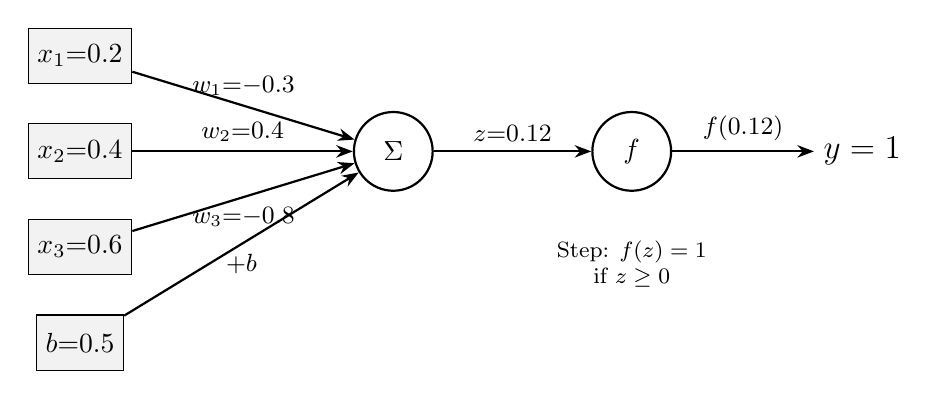
\begin{tikzpicture}[
    node distance=1.6cm and 2.4cm,
    neuron/.style={circle, draw, minimum size=1cm, thick},
    input/.style={rectangle, draw, minimum size=0.7cm, fill=gray!10},
    arr/.style={-{Stealth[length=6pt]}, thick},
    label style/.style={font=\small}
  ]

  %% Input nodes
  \node[input] (x1) {$x_1{=}0.2$};
  \node[input, below=0.5cm of x1] (x2) {$x_2{=}0.4$};
  \node[input, below=0.5cm of x2] (x3) {$x_3{=}0.6$};
  \node[input, below=0.5cm of x3] (b)  {$b{=}0.5$};

  %% Summation node
  \node[neuron, right=2.8cm of x2] (sum) {$\Sigma$};

  %% Activation node
  \node[neuron, right=2.0cm of sum] (act) {$f$};

  %% Output
  \node[right=1.8cm of act, font=\large\bfseries] (out) {$y = 1$};

  %% Arrows from inputs to sum
  \draw[arr] (x1) -- node[above, label style]{$w_1{=}{-}0.3$} (sum);
  \draw[arr] (x2) -- node[above, label style]{$w_2{=}0.4$}   (sum);
  \draw[arr] (x3) -- node[below, label style]{$w_3{=}{-}0.8$} (sum);
  \draw[arr] (b)  -- node[below, label style]{$+b$}           (sum);

  %% Sum to activation
  \draw[arr] (sum) -- node[above, label style]{$z{=}0.12$} (act);

  %% Activation to output
  \draw[arr] (act) -- node[above, label style]{$f(0.12)$} (out);

  %% Step function annotation
  \node[below=0.5cm of act, font=\footnotesize, align=center]
    {Step: $f(z)=1$\\if $z\geq 0$};

\end{tikzpicture}
\caption{Perceptron with bias: three inputs plus a bias unit feeding a
  summation node and a step-function activation.  The bias shifts the
  net input from $-0.38$ to $+0.12$, changing the output from 0 to 1.}
\label{fig:perceptron-bias}
\end{figure}

%% ══════════════════════════════════════════════════════════════════════
\section{Perceptron Convergence and Linear Separability}
\label{sec:convergence}
%% ══════════════════════════════════════════════════════════════════════

\subsection{The Perceptron Convergence Theorem}
\label{subsec:convergence-theorem}

\begin{theorem}[Perceptron Convergence Theorem]
\label{thm:convergence}
If the training data are linearly separable, then the perceptron learning
algorithm (\cref{eq:update}) converges after a finite number of weight
updates.  The resulting weight vector defines a linear hyperplane that
correctly separates all training samples.
\end{theorem}

\begin{remark}
\label{rem:uniqueness}
The theorem guarantees \emph{existence} of a separating hyperplane and
termination in \emph{finite steps}, but it does \emph{not} guarantee
uniqueness.  There may be infinitely many valid separating hyperplanes,
and the algorithm will stop at whichever one it reaches first, depending
on initialisation and sample ordering.
\end{remark}

\subsection{Linear Separability -- Definition}
\label{subsec:linear-separability-def}

\begin{definition}[Linear Separability]
\label{def:linsep}
A set of labelled data points
$\{(\mathbf{x}^{(k)}, d^{(k)})\}_{k=1}^{N}$ with $d^{(k)} \in \{-1, +1\}$
is \emph{linearly separable} if there exists a weight vector $\mathbf{w}$
and bias $b$ such that:
\begin{equation}
  \label{eq:linsep}
  d^{(k)}\!\left(\mathbf{w}^{\top}\mathbf{x}^{(k)} + b\right) > 0
  \quad \forall\, k.
\end{equation}
In two dimensions this means the two classes can be separated by a
straight line; in $M$ dimensions, by a hyperplane.
\end{definition}

\subsection{Boolean Functions and Linear Separability}
\label{subsec:boolean}

For $M = 2$ binary input variables there are $2^{2^M} = 2^4 = 16$
possible Boolean functions.  Of these, \textbf{14 are linearly separable}
and two are not.  \Cref{tab:boolean-gates} summarises the key cases.

\begin{table}[ht]
\centering
\caption{Linear separability of 2-input Boolean functions.}
\label{tab:boolean-gates}
\begin{tabular}{lcccc}
\toprule
\textbf{Function} & \textbf{(0,0)} & \textbf{(0,1)} & \textbf{(1,0)} & \textbf{(1,1)} \\
& output & output & output & output \\
\midrule
AND   & 0 & 0 & 0 & 1 \\
OR    & 0 & 1 & 1 & 1 \\
NAND  & 1 & 1 & 1 & 0 \\
NOR   & 1 & 0 & 0 & 0 \\
\midrule
\textbf{XOR}  & \textbf{0} & \textbf{1} & \textbf{1} & \textbf{0} \\
\textbf{XNOR} & \textbf{1} & \textbf{0} & \textbf{0} & \textbf{1} \\
\bottomrule
\end{tabular}

\vspace{4pt}
\small\textit{Note: XOR and XNOR (bold) are the only non-linearly separable
functions among the 16 two-input Boolean functions.}
\end{table}

\begin{keyinsight}[title=Key Insight -- XOR and XNOR Are Not Linearly Separable]
The XOR function outputs 1 when exactly one input is 1, placing the
positive class at $(0,1)$ and $(1,0)$ and the negative class at $(0,0)$
and $(1,1)$.  Any straight line through the 2-D plane will inevitably
misclassify at least one point.  This is the canonical example motivating
multi-layer networks.  The number of linearly separable functions
\emph{decreases} as input dimensionality $M$ increases.
\end{keyinsight}

\subsection{Decision Boundary Convergence (Figure 4.3)}
\label{subsec:convergence-diagram}

\Cref{fig:convergence} reproduces Figure~4.3 from
B.~Yegnanarayana, \textit{Artificial Neural Networks}, PHI, 1999, showing
how the decision boundary evolves across training epochs $m$ for a
two-class linearly separable dataset.

\begin{figure}[ht]
\centering
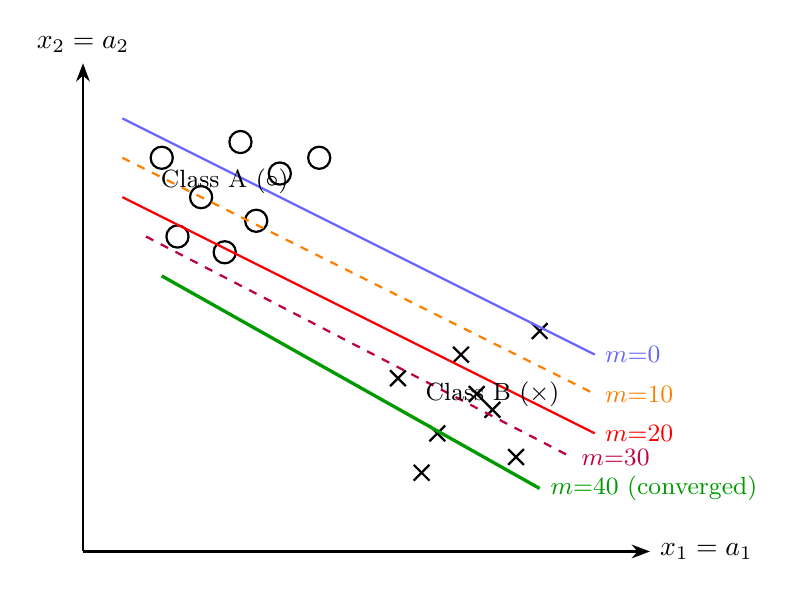
\begin{tikzpicture}[scale=1.0]
  %% Axes
  \draw[-{Stealth}, thick] (0,0) -- (7.2,0) node[right]{$x_1 = a_1$};
  \draw[-{Stealth}, thick] (0,0) -- (0,6.2) node[above]{$x_2 = a_2$};

  %% Class A points (circles) -- upper-left region
  \foreach \x/\y in {1.0/5.0, 1.5/4.5, 2.0/5.2, 1.2/4.0, 2.5/4.8,
                     1.8/3.8, 3.0/5.0, 2.2/4.2}{
    \draw[thick] (\x,\y) circle (4pt);
  }

  %% Class B points (crosses) -- lower-right region
  \foreach \x/\y in {4.5/1.5, 5.0/2.0, 5.5/1.2, 4.8/2.5, 5.2/1.8,
                     4.0/2.2, 5.8/2.8, 4.3/1.0}{
    \draw[thick] (\x-0.1,\y-0.1) -- (\x+0.1,\y+0.1);
    \draw[thick] (\x-0.1,\y+0.1) -- (\x+0.1,\y-0.1);
  }

  %% Decision boundaries at different epochs
  %% m=0
  \draw[blue!60, thick] (0.5,5.5) -- (6.5,2.5)
    node[right, font=\small]{$m{=}0$};
  %% m=10
  \draw[orange, thick, dashed] (0.5,5.0) -- (6.5,2.0)
    node[right, font=\small]{$m{=}10$};
  %% m=20
  \draw[red, thick] (0.5,4.5) -- (6.5,1.5)
    node[right, font=\small]{$m{=}20$};
  %% m=30
  \draw[purple, thick, dashed] (0.8,4.0) -- (6.2,1.2)
    node[right, font=\small]{$m{=}30$};
  %% m=40 (converged)
  \draw[green!60!black, very thick] (1.0,3.5) -- (5.8,0.8)
    node[right, font=\small, text=green!60!black]{$m{=}40$ (converged)};

  %% Class labels
  \node[font=\small] at (1.8,4.7) {Class A ($\circ$)};
  \node[font=\small] at (5.2,2.0) {Class B ($\times$)};

\end{tikzpicture}
\caption{Figure~4.3 (Yegnanarayana, 1999): Decision boundaries produced by
  the perceptron learning algorithm at epochs $m = 0, 10, 20, 30, 40$.
  The boundary wanders until convergence at $m = 40$.  Multiple valid
  boundaries exist; the one reached depends on initialisation.}
\label{fig:convergence}
\end{figure}

\subsection{Perceptron Learning Algorithm}
\label{subsec:algorithm}

\Cref{alg:perceptron} gives the complete training procedure.

\begin{algorithm}[ht]
\caption{Perceptron Learning Algorithm}
\label{alg:perceptron}
\SetAlgoLined
\DontPrintSemicolon
\KwIn{Training set $\{(\mathbf{x}^{(k)}, d^{(k)})\}_{k=1}^{N}$,
      learning rate $\eta > 0$, max epochs $T$}
\KwOut{Weight vector $\mathbf{w}$, bias $w_0$}

Initialise $\mathbf{w} \leftarrow \mathbf{0}$, $w_0 \leftarrow 0$\;
\For{epoch $t = 1$ \KwTo $T$}{
  $\text{errors} \leftarrow 0$\;
  \For{each sample $k = 1$ \KwTo $N$}{
    $z \leftarrow \sum_{i=0}^{n} w_i x_i^{(k)}$ \quad ($x_0^{(k)} \equiv 1$)\;
    $y^{(k)} \leftarrow f(z)$\;
    \If{$y^{(k)} \neq d^{(k)}$}{
      $w_i \leftarrow w_i + \eta\,(d^{(k)} - y^{(k)})\,x_i^{(k)}$
        \quad $\forall\, i$\;
      $\text{errors} \leftarrow \text{errors} + 1$\;
    }
  }
  \If{$\text{errors} = 0$}{
    \textbf{break} \quad (convergence reached)\;
  }
}
\end{algorithm}

\subsection{Multiclass Extension (Figure 4.9)}
\label{subsec:multiclass}

For $C > 2$ linearly separable classes one trains $C$ perceptrons in
parallel, one per class, using a one-versus-all strategy.  The $c$-th
perceptron is trained with samples from class $c$ as positive examples
and all remaining samples as negative examples.

\Cref{fig:multiclass} illustrates the network architecture (Fig.~4.9,
Yegnanarayana, 1999) and the corresponding decision regions for three
classes.

\begin{figure}[ht]
\centering
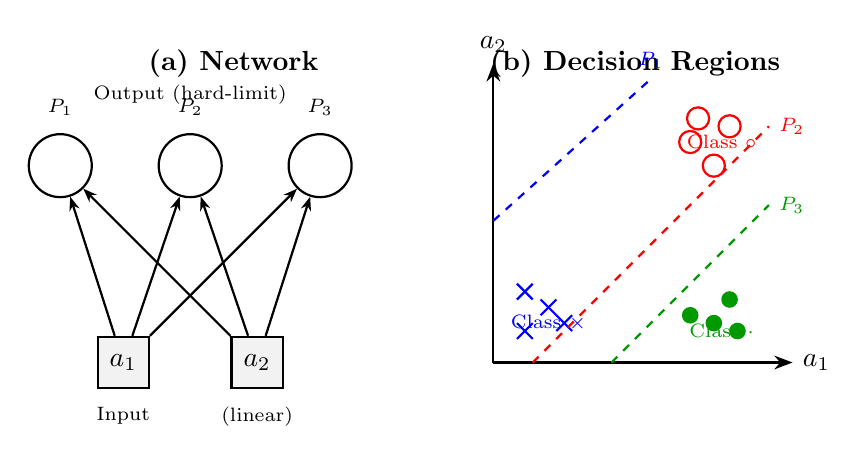
\begin{tikzpicture}[
    node distance=1.2cm and 1.8cm,
    unit/.style={circle, draw, minimum size=0.8cm, thick},
    inp/.style={rectangle, draw, minimum size=0.65cm, fill=gray!10, thick},
    arr/.style={-{Stealth[length=5pt]}, thick}
  ]

  %% ---- (a) Network architecture ----
  \node[font=\bfseries] at (2.2,3.8) {(a) Network};

  %% Input layer
  \node[inp] (a1) at (0.8, 0.0) {$a_1$};
  \node[inp] (a2) at (2.5, 0.0) {$a_2$};
  \node[font=\scriptsize, below=0.1cm of a1] {Input};
  \node[font=\scriptsize, below=0.1cm of a2] {(linear)};

  %% Output layer (3 perceptrons)
  \node[unit] (o1) at (0.0, 2.5) {};
  \node[unit] (o2) at (1.65,2.5) {};
  \node[unit] (o3) at (3.3, 2.5) {};
  \node[font=\scriptsize, above=0.1cm of o1] {$P_1$};
  \node[font=\scriptsize, above=0.1cm of o2] {$P_2$};
  \node[font=\scriptsize, above=0.1cm of o3] {$P_3$};
  \node[font=\scriptsize] at (1.65,3.4) {Output (hard-limit)};

  %% Connections (fully connected)
  \foreach \out in {o1, o2, o3}{
    \draw[arr] (a1) -- (\out);
    \draw[arr] (a2) -- (\out);
  }

  %% ---- (b) Decision regions ----
  \begin{scope}[xshift=5.5cm]
    \node[font=\bfseries] at (1.8,3.8) {(b) Decision Regions};

    \draw[-{Stealth}, thick] (0,0) -- (3.8,0) node[right]{$a_1$};
    \draw[-{Stealth}, thick] (0,0) -- (0,3.8) node[above]{$a_2$};

    %% Class X (crosses) -- lower-left
    \foreach \x/\y in {0.4/0.4, 0.7/0.7, 0.4/0.9, 0.9/0.5}{
      \draw[thick,blue] (\x-0.1,\y-0.1)--(\x+0.1,\y+0.1);
      \draw[thick,blue] (\x-0.1,\y+0.1)--(\x+0.1,\y-0.1);
    }

    %% Class O (circles) -- upper-right
    \foreach \x/\y in {2.5/2.8, 2.8/2.5, 3.0/3.0, 2.6/3.1}{
      \draw[thick,red] (\x,\y) circle (4pt);
    }

    %% Class dot (dots) -- lower-right
    \foreach \x/\y in {2.8/0.5, 3.0/0.8, 2.5/0.6, 3.1/0.4}{
      \fill[green!60!black] (\x,\y) circle (3pt);
    }

    %% Decision boundaries (slant lines)
    \draw[thick, blue,  dashed] (0.0,1.8) -- (2.0,3.6)
      node[above,font=\scriptsize]{$P_1$};
    \draw[thick, red,   dashed] (0.5,0.0) -- (3.5,3.0)
      node[right,font=\scriptsize]{$P_2$};
    \draw[thick, green!60!black, dashed] (1.5,0.0) -- (3.5,2.0)
      node[right,font=\scriptsize]{$P_3$};

    \node[font=\scriptsize,blue]         at (0.7,0.5) {Class $\times$};
    \node[font=\scriptsize,red]          at (2.9,2.8) {Class $\circ$};
    \node[font=\scriptsize,green!60!black] at (2.9,0.4) {Class $\cdot$};
  \end{scope}

\end{tikzpicture}
\caption{Figure~4.9 (Yegnanarayana, 1999): Multiclass perceptron.
  (a)~Network architecture: the input layer contains linear fan-out units;
  the output layer has one hard-limiting perceptron per class.
  (b)~Each perceptron learns a boundary separating its class from all others.}
\label{fig:multiclass}
\end{figure}

\begin{example}[title=Example -- Three-Class One-vs-All Training]
Suppose classes are $\times$, $\circ$, and $\bullet$.  Training proceeds
as follows:
\begin{enumerate}[noitemsep]
  \item Train $P_1$: set $\times$ samples as positive ($d=1$),
        $\circ$ and $\bullet$ as negative ($d=0$).
  \item Train $P_2$: set $\circ$ samples as positive, others as negative.
  \item Train $P_3$: set $\bullet$ samples as positive, others as negative.
\end{enumerate}
At inference, the class with the highest (or the only activated) output
wins.  The method extends to any number of classes, provided all are
linearly separable.
\end{example}

%% ══════════════════════════════════════════════════════════════════════
\section{Linearly Inseparable Problems}
\label{sec:inseparable}
%% ══════════════════════════════════════════════════════════════════════

\subsection{The XOR Problem}
\label{subsec:xor}

The XOR function is the canonical example of a linearly inseparable
problem.  The four data points $(0,0) \to 0$, $(0,1) \to 1$,
$(1,0) \to 1$, $(1,1) \to 0$ cannot be separated by any straight line in
the input plane.

\Cref{tab:xor-vs-or} compares the truth tables of OR and XOR, which have
identical inputs but differ in separability.

\begin{table}[ht]
\centering
\caption{OR (linearly separable) versus XOR (linearly inseparable).}
\label{tab:xor-vs-or}
\begin{tabular}{cc cc cc}
\toprule
\multicolumn{2}{c}{\textbf{Inputs}} & \multicolumn{2}{c}{\textbf{OR output}} & \multicolumn{2}{c}{\textbf{XOR output}} \\
\cmidrule(lr){1-2}\cmidrule(lr){3-4}\cmidrule(lr){5-6}
$x_1$ & $x_2$ & Value & Class & Value & Class \\
\midrule
0 & 0 & 0 & $-$ & 0 & $-$ \\
0 & 1 & 1 & $+$ & 1 & $+$ \\
1 & 0 & 1 & $+$ & 1 & $+$ \\
1 & 1 & 1 & $+$ & 0 & $-$ \\
\bottomrule
\end{tabular}

\vspace{4pt}
\small OR: three positives cluster in one region -- linearly separable.
XOR: positives at $(0,1)$ and $(1,0)$ form a diagonal pattern -- cannot
be enclosed by a single half-plane.
\end{table}

\begin{warningbox}[title=Warning -- Single Perceptron Cannot Solve XOR]
Running the perceptron learning algorithm on XOR data will cause the
decision boundary to wander indefinitely without convergence.  The
Convergence Theorem does not apply because no linearly separating
hyperplane exists.  Attempting to force convergence by capping iterations
will yield a sub-optimal boundary that always misclassifies at least one
sample.
\end{warningbox}

\subsection{Hard Problems and Representation Limits}
\label{subsec:hard-problems}

Problems that are not representable by a single-layer perceptron are
called \emph{hard problems} or \emph{representation problems} in the
neural network literature.  Formally:

\begin{definition}[Hard Problem]
\label{def:hard-problem}
A classification task is a \emph{hard problem} if no linear hyperplane
in the input space separates the classes, i.e., the data are
\emph{linearly inseparable}.
\end{definition}

Key properties of hard problems:
\begin{itemize}[noitemsep]
  \item The perceptron learning algorithm never converges -- the boundary
        oscillates without settling.
  \item The number of linearly separable Boolean functions
        \emph{decreases} as the input dimensionality $M$ increases.
  \item XOR and XNOR are the simplest hard problems for $M = 2$.
\end{itemize}

\subsection{Network Depth vs.\ Decision-Region Complexity (Figure 4.10)}
\label{subsec:depth-vs-region}

A landmark result from Lippmann (1987) -- reproduced in Yegnanarayana
(1999) as Figure~4.10 -- characterises exactly which decision regions
each network depth can realise.

\begin{table}[ht]
\centering
\caption{Decision-region complexity as a function of network depth
  (Lippmann, 1987; Yegnanarayana, 1999, Fig.~4.10).}
\label{tab:depth-regions}
\begin{tabular}{p{3.0cm} p{3.5cm} p{3.5cm} p{3.5cm}}
\toprule
\textbf{Network} & \textbf{Types of decision regions} &
\textbf{XOR problem} & \textbf{Classes with meshed regions} \\
\midrule
Two-layer\\(1 perceptron layer)
  & Half-plane bounded by a single hyperplane
  & Cannot solve (linearly inseparable)
  & Cannot handle \\
\midrule
Three-layer\\(1 hidden layer)
  & Convex open or closed region
  & Solves (convex hull around each class)
  & Cannot handle non-convex \\
\midrule
Four-layer\\(2 hidden layers)
  & Arbitrary region (limited only by neuron count)
  & Solves
  & Handles arbitrary shapes \\
\bottomrule
\end{tabular}
\end{table}

\begin{keyinsight}[title=Key Insight -- Depth Unlocks Richer Decision Regions]
Each additional perceptron layer qualitatively \emph{expands} the class
of representable decision regions.  A two-layer network creates linear
separations only.  A three-layer network combines linear boundaries into
\emph{convex} regions.  A four-layer network combines convex regions into
\emph{arbitrary} (potentially non-convex) shapes.  This hierarchical
composition of simple primitives is the geometric intuition behind the
power of deep networks.
\end{keyinsight}

%% ══════════════════════════════════════════════════════════════════════
\section{Multi-Layer Perceptron: Motivation and Definition}
\label{sec:mlp-motivation}
%% ══════════════════════════════════════════════════════════════════════

\subsection{From Single Layer to Multiple Layers}
\label{subsec:single-to-multi}

The inability of the single perceptron to handle linearly inseparable
data motivated a natural extension: inserting additional layers of
perceptrons \emph{before} the output layer.  Each perceptron in the new
hidden layer learns a linear hyperplane; the output layer then
\emph{combines} these hyperplanes into a more complex surface.

Formally, if the first perceptron layer produces outputs
$\mathbf{h} = (h_1, h_2, \ldots, h_p)$, the output layer operates on
$\mathbf{h}$ rather than the raw input $\mathbf{x}$:

\begin{align}
  \label{eq:mlp-forward}
  h_j &= f\!\left(\sum_{i=0}^{n} w_{ji}^{(1)} x_i\right),
    \quad j = 1, \ldots, p, \\[4pt]
  y_c &= f\!\left(\sum_{j=0}^{p} w_{cj}^{(2)} h_j\right),
    \quad c = 1, \ldots, C.
\end{align}

\subsection{Geometric Intuition}
\label{subsec:geometric-intuition}

Each hidden-layer perceptron creates a linear half-plane in the input
space.  The output perceptron performs a logical AND-like combination of
these half-planes, yielding a \emph{convex} region.  Two hidden layers
allow the second hidden layer to combine convex regions, producing
\emph{non-convex} or even disjoint regions.

As stated in the lecture:
\begin{quote}
\textit{``If I combine the outputs of two or more perceptrons in the next
perceptron layer, you get a modified hyper surface.  Convex surfaces will
be created.  The intersection of convex regions may produce any non-convex
region also.''}
\end{quote}

\begin{definition}[Convex Region]
\label{def:convex}
A region $\mathcal{R} \subseteq \mathbb{R}^n$ is \emph{convex} if for
every two points $\mathbf{p}, \mathbf{q} \in \mathcal{R}$, the line
segment $\lambda\mathbf{p} + (1-\lambda)\mathbf{q}$ for
$\lambda \in [0,1]$ lies entirely within $\mathcal{R}$.
\end{definition}

\subsection{MLP Architecture Diagram}
\label{subsec:mlp-diagram}

\Cref{fig:mlp} shows the four-layer feedforward network that can handle
arbitrary decision regions.

\begin{figure}[ht]
\centering
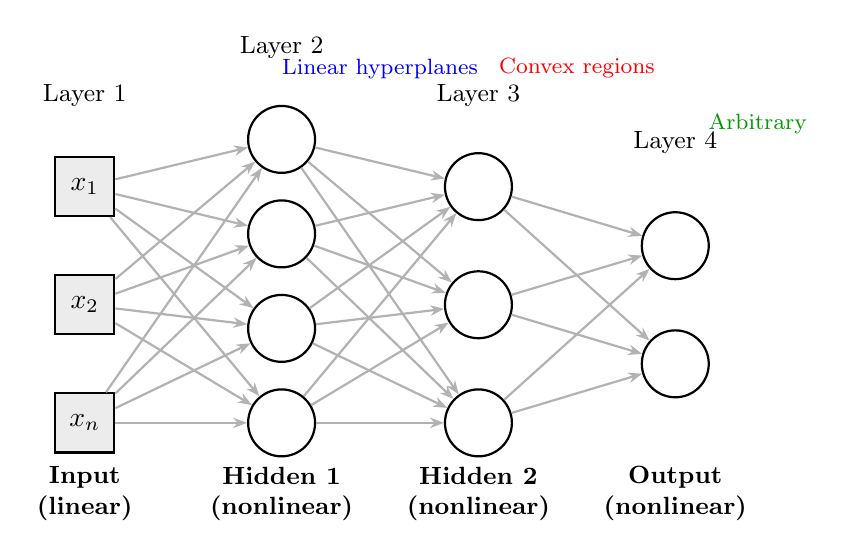
\begin{tikzpicture}[
    unit/.style={circle, draw, minimum size=0.85cm, thick, fill=white},
    inp/.style={rectangle, draw, minimum size=0.75cm, fill=gray!15, thick},
    arr/.style={-{Stealth[length=5pt]}, thick, gray!60},
    labl/.style={font=\small\bfseries, align=center}
  ]

  %% Layer positions (x-coords)
  \def\xI{0}
  \def\xH{2.5}
  \def\xHH{5.0}
  \def\xO{7.5}

  %% Input layer (3 units)
  \foreach \y/\name in {3.0/x1, 1.5/x2, 0.0/x3}{
    \node[inp] (\name) at (\xI, \y) {};
  }
  \node[inp] (x1l) at (\xI, 3.0) {$x_1$};
  \node[inp] (x2l) at (\xI, 1.5) {$x_2$};
  \node[inp] (x3l) at (\xI, 0.0) {$x_n$};
  \node[labl] at (\xI, -0.9) {Input\\(linear)};

  %% Hidden layer 1 (4 units)
  \foreach \y/\name in {3.6/h11, 2.4/h12, 1.2/h13, 0.0/h14}{
    \node[unit] (\name) at (\xH, \y) {};
  }
  \node[labl] at (\xH, -0.9) {Hidden 1\\(nonlinear)};

  %% Hidden layer 2 (3 units)
  \foreach \y/\name in {3.0/h21, 1.5/h22, 0.0/h23}{
    \node[unit] (\name) at (\xHH, \y) {};
  }
  \node[labl] at (\xHH, -0.9) {Hidden 2\\(nonlinear)};

  %% Output layer (2 units)
  \foreach \y/\name in {2.25/o1, 0.75/o2}{
    \node[unit] (\name) at (\xO, \y) {};
  }
  \node[labl] at (\xO, -0.9) {Output\\(nonlinear)};

  %% Connections Input -> H1
  \foreach \s in {x1l, x2l, x3l}{
    \foreach \t in {h11, h12, h13, h14}{
      \draw[arr] (\s) -- (\t);
    }
  }

  %% Connections H1 -> H2
  \foreach \s in {h11, h12, h13, h14}{
    \foreach \t in {h21, h22, h23}{
      \draw[arr] (\s) -- (\t);
    }
  }

  %% Connections H2 -> Output
  \foreach \s in {h21, h22, h23}{
    \foreach \t in {o1, o2}{
      \draw[arr] (\s) -- (\t);
    }
  }

  %% Layer labels
  \node[font=\small, above=0.3cm] at (\xI,  3.6) {Layer 1};
  \node[font=\small, above=0.3cm] at (\xH,  4.2) {Layer 2};
  \node[font=\small, above=0.3cm] at (\xHH, 3.6) {Layer 3};
  \node[font=\small, above=0.3cm] at (\xO,  3.0) {Layer 4};

  %% Brace annotations
  \node[font=\footnotesize, blue, align=center] at (3.75, 4.5)
    {Linear hyperplanes};
  \node[font=\footnotesize, red,  align=center] at (6.25, 4.5)
    {Convex regions};
  \node[font=\footnotesize, green!60!black, align=center, right] at (7.8, 3.8)
    {Arbitrary};

\end{tikzpicture}
\caption{Four-layer feedforward network (Multi-Layer Perceptron).
  Layer 1 (input) distributes data; Layer 2 (first hidden) creates linear
  hyperplanes; Layer 3 (second hidden) combines them into convex regions;
  Layer 4 (output) further combines these into arbitrary decision regions.}
\label{fig:mlp}
\end{figure}

\begin{definition}[Multi-Layer Perceptron (MLP)]
\label{def:mlp}
A \emph{Multi-Layer Perceptron} is a fully connected feedforward neural
network consisting of:
\begin{itemize}[noitemsep]
  \item An \emph{input layer} of linear fan-out units (not counted as a
        perceptron layer);
  \item One or more \emph{hidden layers} of nonlinear perceptrons;
  \item An \emph{output layer} of nonlinear perceptrons.
\end{itemize}
A network with three or more total layers (i.e., two or more perceptron
layers) is called a multi-layer perceptron.
\end{definition}

\subsection{Relationship Between Layers and Region Complexity}
\label{subsec:layers-regions}

\begin{theorem}[Layer-Region Correspondence]
\label{thm:layers-regions}
For a feedforward network with hard-limiting (step function) units:
\begin{itemize}[noitemsep]
  \item \textbf{1 perceptron layer} (2-layer network): produces linear
        hyperplane boundaries -- half-plane regions only.
  \item \textbf{2 perceptron layers} (3-layer network): produces
        convex regions formed by the intersection of linear hyperplanes.
  \item \textbf{3 perceptron layers} (4-layer network): produces
        arbitrary regions formed by the union of convex regions.
\end{itemize}
\end{theorem}

The theorem also holds when the step function is replaced by a continuous
nonlinear activation (e.g., sigmoid), as noted by the instructors:
``Similar behavior is expected from a multi-layer feed-forward network
when the output functions of the units are continuous non-linear
functions, such as sigmoid.''

\subsection{Number of Units and Surface Complexity}
\label{subsec:unit-count}

Key design parameters govern the expressiveness of the network:

\begin{itemize}[noitemsep]
  \item The number of units in the \textbf{first hidden layer} determines
        the \emph{shape} of the dividing surfaces (how many hyperplane
        ``facets'' can be combined).
  \item The number of units in the \textbf{output layer} determines the
        \emph{number of classes} the network can discriminate.
  \item Adding more units to the hidden layers increases the complexity
        of achievable decision boundaries.
\end{itemize}

%% ══════════════════════════════════════════════════════════════════════
\section{The Problem with the Perceptron}
\label{sec:problem}
%% ══════════════════════════════════════════════════════════════════════

\subsection{Non-Uniqueness of the Separating Hyperplane (V06)}
\label{subsec:non-unique}

Even when the data \emph{are} linearly separable, the perceptron has a
fundamental limitation: it finds \emph{some} separating hyperplane, but
has \emph{no mechanism} to select the \emph{best} one.

As illustrated in the lecture (timestamp 01:05:00), infinitely many valid
hyperplanes A, B, C, D can all separate the two classes, yet the
perceptron stops at whichever it encounters first.

\begin{align}
  \label{eq:loss-hinge}
  \mathcal{L}_{\text{hinge}}(\mathbf{w}) =
  \sum_{k=1}^{N} \max\!\bigl(0,\; -\,y^{(k)}\,\mathbf{w}^{\top}\mathbf{x}^{(k)}\bigr),
\end{align}

where $y^{(k)} \in \{-1, +1\}$.  The perceptron loss is zero for any
correctly separating hyperplane regardless of the margin -- it cannot
distinguish between a boundary that passes close to the data and one that
has a wide margin.

\subsection{Contrast with Support Vector Machines}
\label{subsec:svm-comparison}

A student question during the lecture highlighted an important contrast:

\begin{quote}
\textit{Student: ``In SVM we select a hyperplane that maximises the
margin.  Does the perceptron also maximise the margin?''}

\textit{Instructor: ``Here it is not a maximum margin classifier.
That is where I told you, there are infinite solutions possible.  For a
maximum margin classifier, the line should come exactly in the centre so
that all the samples are equally distanced from positive and negative
examples.  In the neural network, there is no maximum margin classifier.''}
\end{quote}

\Cref{tab:perceptron-svm} contrasts the two approaches.

\begin{table}[ht]
\centering
\caption{Perceptron vs.\ Support Vector Machine (SVM).}
\label{tab:perceptron-svm}
\begin{tabular}{lll}
\toprule
\textbf{Property} & \textbf{Perceptron} & \textbf{SVM} \\
\midrule
Objective          & Correct classification & Maximum margin \\
Solution uniqueness & Any valid boundary     & Unique (maximum-margin) \\
Optimality         & No guarantee           & Optimal (max margin) \\
Convergence        & Finite if separable    & Always (via QP) \\
Non-linear case    & Needs MLP / more layers & Kernel trick \\
Update rule        & Perceptron rule        & Quadratic programming \\
\bottomrule
\end{tabular}
\end{table}

\begin{keyinsight}[title=Key Insight -- Perceptron Finds a Solution but Not the Best]
The perceptron's lack of a margin optimisation criterion is one of its
principal weaknesses.  This limitation motivated two parallel lines of
research: (1) the Support Vector Machine, which explicitly maximises the
margin, and (2) gradient-based training of multi-layer networks with
differentiable loss functions, which can be designed to prefer
well-generalising solutions.
\end{keyinsight}

%% ══════════════════════════════════════════════════════════════════════
\section{Activation Functions}
\label{sec:activations}
%% ══════════════════════════════════════════════════════════════════════

\subsection{Overview}
\label{subsec:activations-overview}

The activation function $f$ transforms the weighted sum $z =
\sum_i w_i x_i + b$ into the neuron's output.  Although the classical
perceptron uses the step function, the lecture introduces several
alternatives that make the model more flexible and differentiable.

\subsection{Step Function}
\label{subsec:step}

\begin{equation}
  \label{eq:step-fn}
  f_{\text{step}}(z) =
  \begin{cases}
    1 & z \geq 0, \\
    0 & z < 0.
  \end{cases}
\end{equation}

Output: $\{0, 1\}$.  Non-differentiable at the origin; used in the
classical perceptron.

\subsection{Sigmoid Function}
\label{subsec:sigmoid}

\begin{equation}
  \label{eq:sigmoid}
  f_{\sigma}(z) = \frac{1}{1 + e^{-z}}.
\end{equation}

Output: $(0, 1)$ -- interpretable as a probability.  Differentiable
everywhere; the ``S-shaped'' curve is bounded and monotone.  Preferred
when probabilistic outputs are required.

\subsection{Hyperbolic Tangent}
\label{subsec:tanh}

\begin{equation}
  \label{eq:tanh}
  f_{\tanh}(z) = \tanh(z) = \frac{e^{z} - e^{-z}}{e^{z} + e^{-z}}.
\end{equation}

Output: $(-1, +1)$.  Zero-centred, which can speed up training.
Commonly used in recurrent neural networks (LSTMs, GRUs) for hidden-state
activations.

\subsection{Rectified Linear Unit (ReLU)}
\label{subsec:relu}

\begin{equation}
  \label{eq:relu}
  f_{\text{ReLU}}(z) = \max(0, z).
\end{equation}

Output: $[0, \infty)$.  Computationally efficient; avoids vanishing
gradients for positive inputs.  Widely used in convolutional neural
networks (CNNs).

\begin{table}[ht]
\centering
\caption{Comparison of common activation functions.}
\label{tab:activations}
\begin{tabular}{lcccc}
\toprule
\textbf{Function} & \textbf{Formula} & \textbf{Range} &
\textbf{Differentiable} & \textbf{Typical use} \\
\midrule
Step     & $\mathbf{1}[z \geq 0]$             & $\{0,1\}$   & No (at 0) & Classical perceptron \\
Sigmoid  & $1/(1+e^{-z})$                      & $(0,1)$     & Yes       & Binary classification \\
Tanh     & $(e^z - e^{-z})/(e^z + e^{-z})$    & $(-1,1)$    & Yes       & RNNs, LSTMs \\
ReLU     & $\max(0, z)$                        & $[0,\infty)$& No (at 0) & CNNs, deep networks \\
\bottomrule
\end{tabular}
\end{table}

\begin{example}[title=Example -- Sigmoid vs.\ Step on the Same Input]
Consider $z = 0.12$ (from the bias example in \cref{sec:bias}).
\begin{align*}
  f_{\text{step}}(0.12)   &= 1, \\
  f_{\sigma}(0.12)         &= \frac{1}{1 + e^{-0.12}} \approx 0.530, \\
  f_{\tanh}(0.12)          &= \tanh(0.12) \approx 0.119, \\
  f_{\text{ReLU}}(0.12)   &= 0.12.
\end{align*}
The step function gives a hard binary decision.  The sigmoid provides a
probability near 0.53, reflecting mild confidence.  Tanh gives a
zero-centred near-zero output.  ReLU passes the value through unchanged
(since it is positive).
\end{example}

%% ══════════════════════════════════════════════════════════════════════
\section{Summary and Conclusion}
\label{sec:conclusion}
%% ══════════════════════════════════════════════════════════════════════

\subsection{Session Summary}
\label{subsec:summary}

Session~04 completed the perceptron coverage and laid the conceptual
groundwork for Multi-Layer Perceptrons.  The key results are:

\begin{enumerate}[label=\textbf{\arabic*.}, noitemsep]
  \item \textbf{Bias is a learned parameter.}  It shifts the decision
        boundary away from the origin, enabling classification of patterns
        that pure weighted sums cannot handle.

  \item \textbf{The Perceptron Convergence Theorem.}  For linearly
        separable data, the perceptron learning algorithm converges in a
        finite number of steps to a valid separating hyperplane.

  \item \textbf{XOR and XNOR are not linearly separable.}  Of the 16
        two-input Boolean functions, only these two cannot be learned by a
        single perceptron.  The number of linearly separable functions
        decreases as dimensionality increases.

  \item \textbf{The perceptron finds a boundary but not the best one.}
        There are infinitely many valid separating hyperplanes; the
        perceptron has no margin-optimisation mechanism.

  \item \textbf{Depth enables richer decision regions.}  Two-layer
        networks create half-planes; three-layer networks create convex
        regions; four-layer networks create arbitrary regions
        (Lippmann, 1987).

  \item \textbf{MLP as the solution to hard problems.}  Multi-Layer
        Perceptrons with two or more hidden perceptron layers can
        represent any decision region and are not limited to linearly
        separable tasks.

  \item \textbf{Activation function flexibility.}  By replacing the step
        function with sigmoid, tanh, or ReLU, the same network
        architecture can be used for probability estimation, zero-centred
        regression, or sparse activation respectively.
\end{enumerate}

\subsection{Looking Ahead}
\label{subsec:ahead}

The conceptual framework established here -- that depth unlocks
expressiveness -- is the foundation of all modern deep learning.  The
next challenge, addressed in subsequent sessions, is \emph{how to train}
a multi-layer network.  The perceptron learning rule does not extend
directly to hidden layers (there is no desired output to compare against
for intermediate nodes).  The solution is \textbf{backpropagation} with
gradient-based optimisation, which uses the chain rule to propagate error
signals from the output back through all hidden layers.

\begin{keyinsight}[title=Key Insight -- The Road from Perceptron to Deep Learning]
The perceptron story -- simple model, guaranteed convergence for easy
problems, fundamental limitation for hard problems -- is a microcosm of
the entire history of machine learning.  Every advance in deep learning
(MLPs, CNNs, RNNs, Transformers) can be read as a response to a specific
limitation of simpler models.  Understanding why a perceptron \emph{fails}
on XOR is therefore not just a historical curiosity: it is the seed from
which the entire field grew.
\end{keyinsight}

%% ══════════════════════════════════════════════════════════════════════
%%  REFERENCES
%% ══════════════════════════════════════════════════════════════════════
\newpage
\begin{thebibliography}{9}

\bibitem{yegna1999}
B.~Yegnanarayana,
\textit{Artificial Neural Networks},
PHI Learning, New Delhi, 1999.

\bibitem{lippmann1987}
R.~P.~Lippmann,
``An introduction to computing with neural nets,''
\textit{IEEE ASSP Magazine}, vol.~4, no.~2, pp.~4--22, Apr.~1987.

\bibitem{rosenblatt1958}
F.~Rosenblatt,
``The perceptron: A probabilistic model for information storage and
organization in the brain,''
\textit{Psychological Review}, vol.~65, no.~6, pp.~386--408, 1958.

\bibitem{minsky1969}
M.~Minsky and S.~Papert,
\textit{Perceptrons: An Introduction to Computational Geometry},
MIT Press, Cambridge, MA, 1969.

\bibitem{rumelhart1986}
D.~E.~Rumelhart, G.~E.~Hinton, and R.~J.~Williams,
``Learning representations by back-propagating errors,''
\textit{Nature}, vol.~323, pp.~533--536, 1986.

\end{thebibliography}

\end{document}
